\chapter{e1000 paravirtualization}
\label{cha:paravirt}
In chapter \ref{cha:e1000-opt} we have proposed two simple patches that boost the e1000 performances.
The moderation patch involves only modification to the hypervisor, while the batching patch involves only modification to the
guest device driver. These patches cannot be applied independently on each other, even if the batching generally works better if
it comes together with moderation.

Neverthless, in both cases the we have respected the original e1000 specification, so that the guest can use the e1000 adapter with its
original (or patched) driver and be unaware that it is actually in a Virtual Machine environment, and that the e1000 adapter is
emulated. This unawareness is the essence of the \emph{full virtualization} concept: The guest doesn't know to be emulated, so
that we can run an unmodified OS on top of it and everything works fine.

\vspace{0.5cm}

Another approach that sometimes is used is \emph{paravirtualization}, a general concept that describes situations in which the 
guest is aware of being in a Virtual Machine environment, and cooperates with the hypervisor in order to make the virtualization simpler
and/or to get better performances.


\section{Device paravirtualization}
In this thesis we are interested in device paravirtualization, and in particular in network device paravirtualization.
With this kind of paravirtualization, only the \emph{paravirtualized} device driver is aware of the virtualization, while the rest of the
system is not.
We can obtain a paravirtualized driver either by modifying an existing real driver, or by creating a new \emph{fake} driver. In the
latter case the driver correspond to a new virtual (fake) device that does not really exist, but is just a stub used to communicate with 
the outside world exporting to the guest OS the same interface exported by a real driver, so that the guest OS
can make use of it without being aware that the device is a fake one.
In both cases the paravirtualization requires hypervisor support.

In our case we could modify the e1000 Linux driver and the e1000 QEMU frontend, or we could create a new Linux network driver and
a new QEMU frontend.

\vspace{0.5cm}

How can paravirtualization improve performances? Device hardware specifications are generally very complex, and often
inlcude a lot of physical details, offloading capabilities and other hardware related features. When emulating the device, most of these 
details and features are just useless, or is not worth/possible implementing it. Moreover, the devices communicate with the OS mainly 
through register accesses because register accesses are not expensive in hardware, but they do are expensive within emulators, since
they cause VMExits. In other words, emulating real device is complicated and inefficient.

\vspace{0.5cm}

The idea behind paravirtualization is that most of hardware-related details are source of useless overhead, and this overhead can be 
easily avoided if the driver knows that it is talking to a virtual device and not to a real hardware. As an example, the e1000 driver has
to do at least 5 VMExit while executing the interrupt routine, but if we knew that the e1000 device is virtual, some (or all) of these
would become useless, or at least could be replaced with something cheaper.

The purpose of a paravirtualized devices is therefore to estabilish an efficient communication between the device driver and the emulator
(e.g. the QEMU frontend), while the guest OS think of the driver as being a driver of a real device.
In order to make the communication efficient, we have to minimize VMExits, and so register accesses. The communication should be done, when
possible, through shared memory. The TX ring is an example of shared memory used for communication: The driver writes to the TX ring and
the frontend reads from it (and then also writes back). The RX ring is another example.

However, also a paravirtualized driver needs to access register, since a register access is the only way the driver can notify the
emulator to start some processing or, in general, to have side effects. The difference with a real driver is that a paravirtualized one
does a register access only when is really essential, e.g. for notifications. For everything else, the communication is done through
shared memory. A real device driver doesn't worry so much about accessing registers.



\section{The Virtio standard}
Virtio is a virtualization standard that aims at high I/O performances through device paravirtualization. This is done creating completely
new device drivers, which are able to communicate efficiently with a Virtio-capable hypervisor. Its approach is
similar to the Xen I/O paravirtualization and the VMware \emph{Guest Tools}.
Virtio is an effort to estabilish a standard interface between drivers and hypervisors for paravirtualized I/O, in order to increase the 
code reuse across platform. In this way we avoid to have an independent I/O paravirtualization solution for each hypervisor.
The Virtio standard defines different I/O (fake) devices, including a network adapter, a SCSI disk and a serial interface, and is currently
supported by QEMU and Virtualbox. Linux and Windows drivers are available for Virtio devices.

\begin{figure}[bt]
\centering
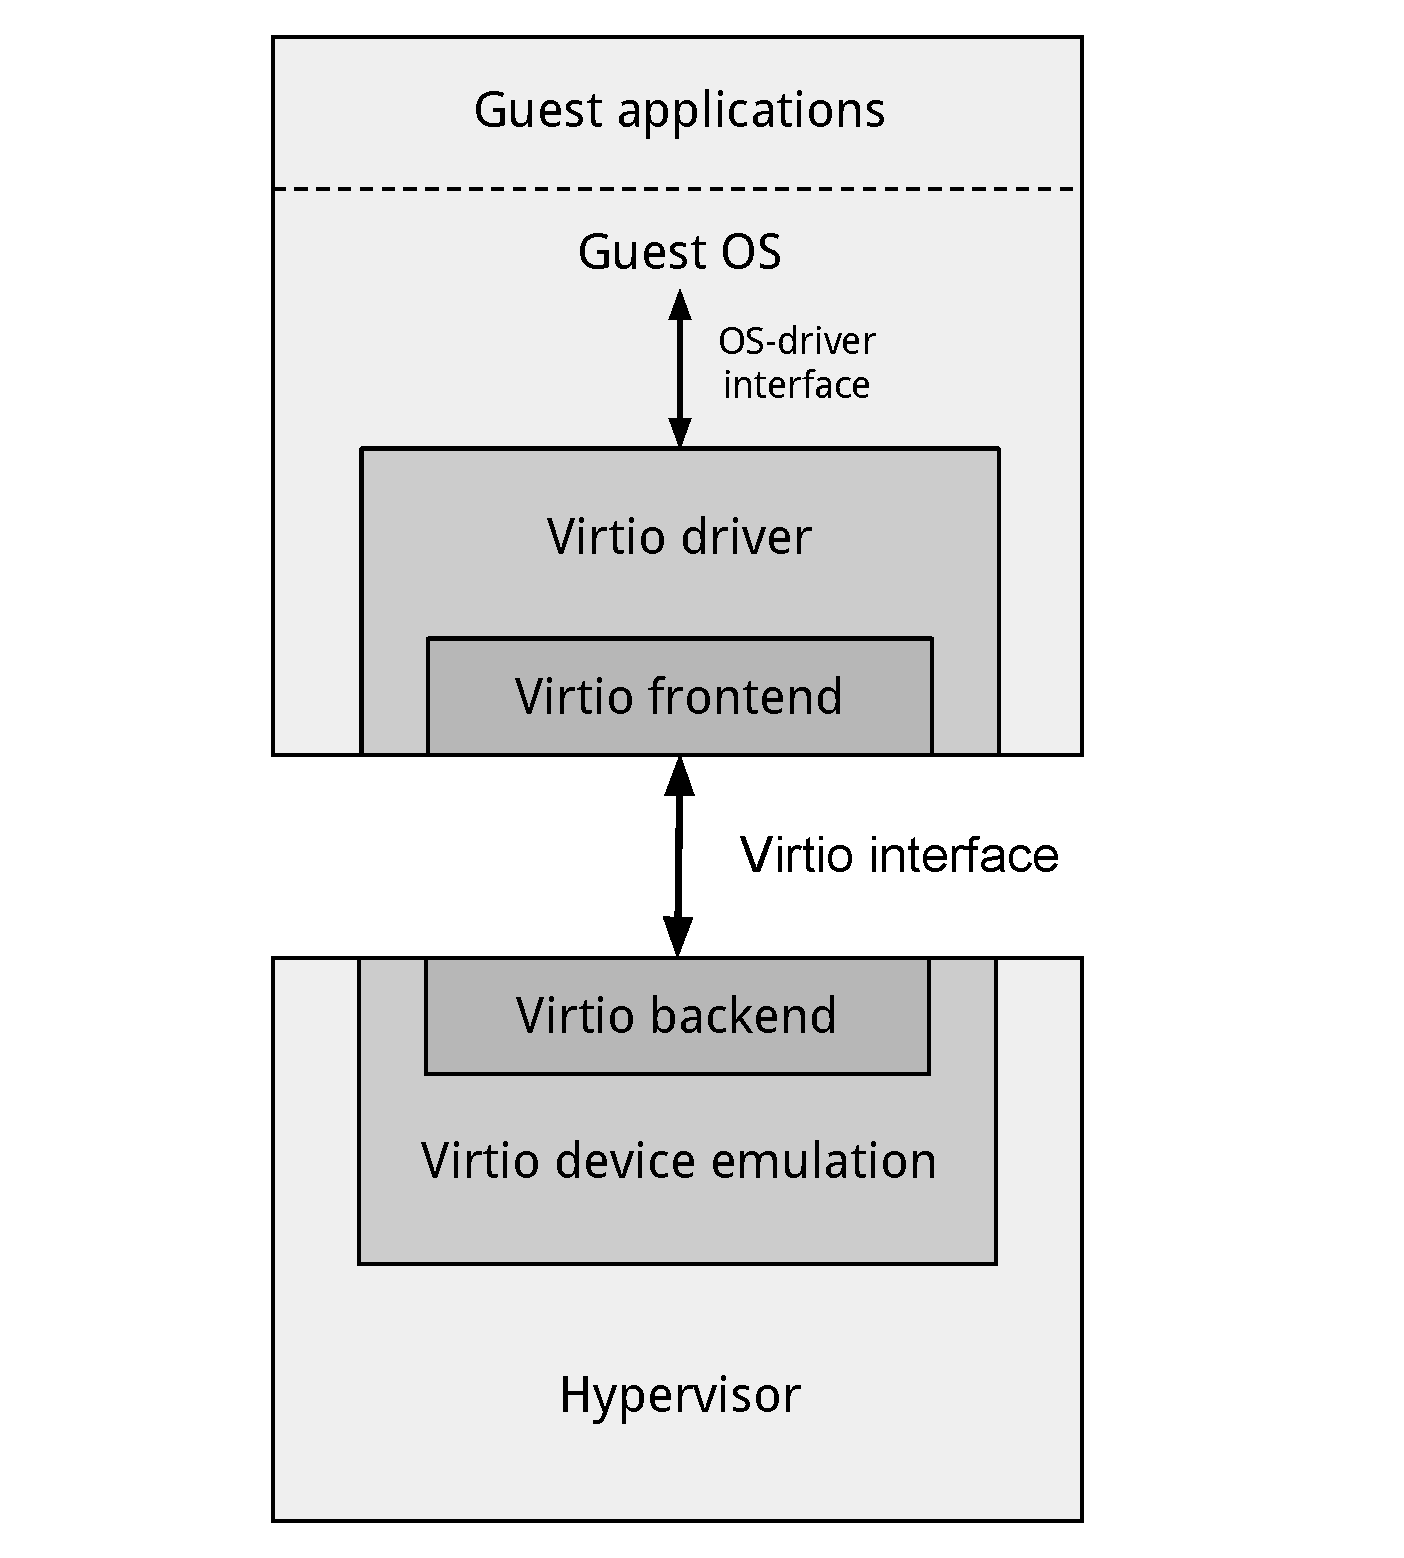
\includegraphics[scale = 0.45]{virtio.pdf}
\caption{A guest and its hypervisor communicate through the Virtio interface.}
\label{fig:virtio}
\end{figure}

As we can see from figure \ref{fig:virtio}, the Virtio interface is implemented through a virtio frontend in the guest OS, and a virtio
backend in the hypervisor. All the virtio device drivers can share the virtio frontend code. The task of a virtio driver is therefore to
convert the OS representation of the data to exchange (e.g. a network packet) into the standard virtio data format, or the other way
around. All the virtio device emulators (e.g. the QEMU frontend for each virtio device) can share the virtio backend code. The task
of a virtio device emulator is therefore to convert the virtio representation of the data to exchange into the hypervisor specific
representation (e.g. a buffer containg an ethernet frame), or the other way around. In this way, the guest OS and the hypervisor can
communicate through the virtio infrastructure using an efficient and general mechanism.

\vspace{0.5cm}

The organization illustrated in figure \ref{fig:virtio} is actually similar to the one used for real device emulation (e.g. e1000 standard).
However the Virtio interface is explicitely designed for efficient communication between driver and hypervisor, while this is not true for
real device hardware/software interfaces.


\subsection{Virtual queues}
\label{sec:virtqueue}
Central to the Virtio interface is the \emph{virtual queue} abstraction, a queue that connects a virtio frontend to a virtio backend.
A virtual queue is simply a queue into which buffers are posted by the guest driver for consumption by the hypervisor: In this way
the two peers can exchange data.
A virtual queue can be used to exchange data in both directions: Therefore the posted buffers can be used both for output and for input 
operations. Drivers can use zero, one or more queues, depending on their needs. For example, the virtio network device uses two virtual
queues (one for receive and one for transmit), while the virtio block device uses only one.
The buffers use to exchange data are represented in Virtio using scatter-gather lists\footnote{Each
element in the list represents the guest physical address and a length of a physical contiguous chunk of memory}. With a single operation
a virtio frontend can send a scatter-gather list to a virtio backend. A single scatter-gather list can specify both input and output 
requests. For example, the guest may send to the hypervisor a SG-list containing three buffers: An output buffer that specifies a 
command and two input buffer that will be filled by the hypervisor with the response\footnote{This example could be valid for a virtio
disk.}.

\vspace{0.5cm}

In more detail, when the guest wants to make requests to the hypervisor through a virtual queue, it invokes the \texttt{add\_buf} method
on the virtual queue object, passing a SG-list and a non-NULL token which is returned when the SG has been consumed. As we have seen 
previously, a single SG-list can be used to pass many output buffers (e.g. network packets to send) and many input buffers (e.g. memory 
buffers where the hypervisor can store received network packets). The method returns the amount of space left in the queue, so that 
the guest can stop adding new buffers when the queue is full.
The \texttt{add\_buf} method doesn't notify the hypervisor about the new requests, but only inserts the new buffer in the ring associated
with the virtual queue object. When a virtio driver wants to notify the hypervisor, it has to call the \texttt{kick} method. Of course
the driver should kick the hypervisor only when necessary, and try to add as many buffers as possible before \emph{kicking} the hypervisor.

When the hypervisor is notified, it extracts (pops) an SG list from the virtual queue and process the request, maybe asynchronously.
When the processing is done, the hypervisor returns the used SG list to the virtual queue.
The guest can poll for the request completion through the \texttt{get\_buf} function. This function is not blocking and returns NULL if 
there are no returned used SG lists, or returns the token of a SG list that has been consumed.
The whole process is depicted in figure \ref{fig:virtqueue}.

\begin{figure}[bt]
\centering
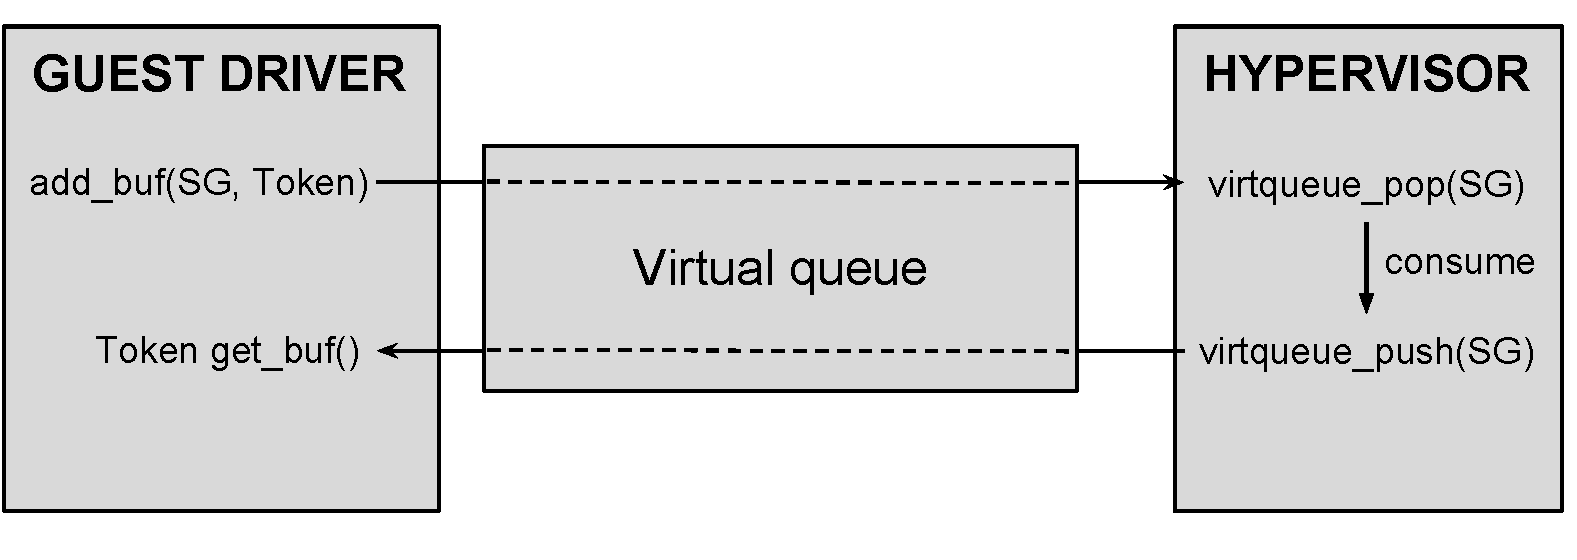
\includegraphics[scale = 0.48]{virtqueue.pdf}
\caption{Virtual queue operations.}
\label{fig:virtqueue}
\end{figure}

\vspace{0.5cm}

In order to avoid busy waiting, the driver can provide a callback function to a virtual queue. This callback will be invoked when the
hypervisor notifies that new used buffers have been returned. Since hypervisor notifications are generally expensive (in QEMU-KVM they are 
implemented as interrupts to the guest, so they are extremely expensive), the driver should implement strategies aimed at mitigating the
notification rate (e.g. with NAPI). In order to do that, the driver can enable or disable callbacks (e.g. enable/disable interrupts) 
invoking the \texttt{enable\_cb} or \texttt{disable\_cb} methods on the virtual queue. The \texttt{disable\_cb} is actually only a hint,
there is no guarantee that the callback will not still be called right after, since this would require expensive synchronization: It is
just an optimization to reduce unnecessary notifications.
The callback function can call the \texttt{get\_buf} so that it can process the used buffers.


\subsection{The virtio ring transport mechanism}
In the current implementation, the virtual queues are implemented as \emph{rings}, similarly to what happens with network adapters (see
section \ref{sec:e1000-interface}). The Virtio interface hides the rings, so that we could use a different implementation as
long as both virtio frontend and virtio backend use the same transport mechanism.
Since a virtio ring must be a very general and flexible mechanism for transporting buffers, it is also quite complex, or at least more
complex than needed for and efficient paravirtualized network device.

\vspace{0.5cm}

A virtio ring consists of three parts: the descriptor array where the guest chains together length/address pairs (taken from a guest-provided
SG list), the \emph{available} ring where the guest indicates what descriptors chains are ready for use, and the \emph{used} ring where the
host indicates which descriptors chains it has used. Each descriptor contains the guest-physical address of the buffer, its length, an 
optional \texttt{next} index for buffer chaining, and two flags: one to indicate whether the next field is valid and one controlling 
whether the buffer is read-only or write-only. This allows a chained buffer to contain both readable and writable parts (this is 
useful for implementing a block device).
The available ring consists of a free-running index (the \emph{avail} index)\footnote{The ring index is a 16 bit unsigned integer, 
which is always incremented and is intended to overflow.}, an interrupt suppression flag, and an array of indices into the descriptor array 
where each index references the head of a descriptor chains. As we can see, the available ring is separated from the descriptor array, 
adding another level of indirection: The avail index references an entry of the avail ring and this entry references an entry of the
descriptor array (an head of a descriptor chain).
This separation of the descriptor array from the available ring is due to the asynchronous nature of the virtqueue. In fact the hypervisor
extracts the chains in the same order in which they have been inserted, but may process them in a different order and/or asynchronously.
In this case some chains could require more time than others, and so the available ring could circle many times with fast-serviced
chains while slow descriptors might still await completion (this is useful for block device implementation).
The interrupt suppression flag is set when the virtio driver invokes the \texttt{disable\_cb} and is suppressed when the
\texttt{enable\_cb} is invoked. In this way the guest can implement a mitigation strategy for host notification (section 
\ref{sec:virtqueue}).
The used ring has the same structure of the the available ring, but is written by the host as descriptor chains are consumed. Moreover,
the each entry of used ring contains not only an index in the descriptor array, but also a \texttt{len} field which is used for input
buffers: When an input buffer has been used, the hypervisor writes in this field the size of the read operation which wrote to the buffer.

The data structures are depicted in figure \ref{fig:vring}.

\begin{figure}[bt]
\centering
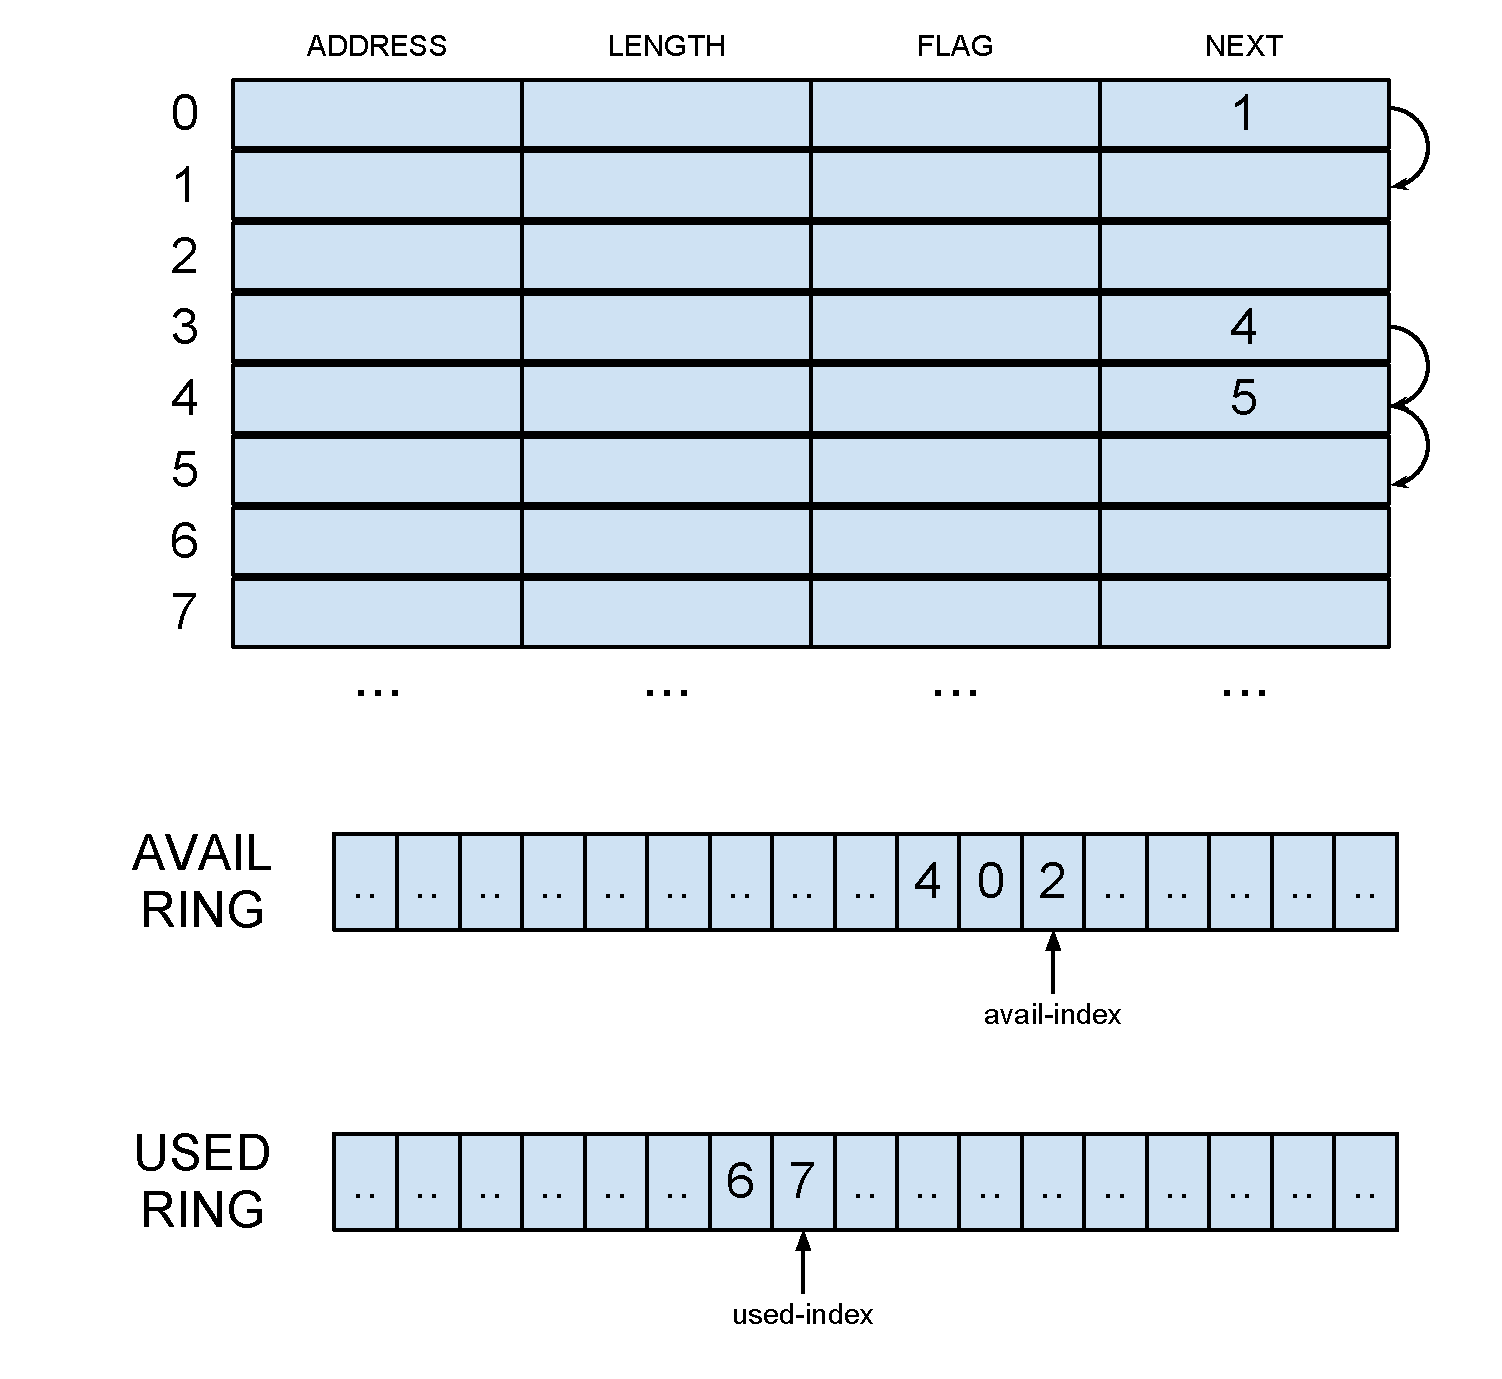
\includegraphics[scale = 0.48]{vring.pdf}
\caption{Virtio ring structures. On the top the descriptor array is depicted as a table. On the bottom the \emph{avail} ring and the 
	 \emph{used} ring.}
\label{fig:vring}
\end{figure}

\vspace{0.5cm}

Putting all together, let's describe the journey of a virtio buffer in a virtual queue. A virtio driver invokes \texttt{add\_buf} on the
virtual queue, and the provided SG list is inserted in the descriptor array, using a free entry for each element in the SG list. All this
descriptors are chained together. At this point a new entry is inserted in the avail ring, referencing the head of the chain just now
built, and the avail index is incremented.
Now the virtio driver can kick the hypervisor (if is the case), because there is a new entry in the avail ring.
When the hypervisor sees that there is work to do, it pops the new entry from the available ring, processes it, pushes the used descriptor
chain in the used ring, increments the used index and, if is the case, notifies the guest (e.g. send an interrupt). When the guest wants 
to get an used buffer, it invokes the \texttt{get\_buf} method so that it can clean or complete to process the returned buffer.


\subsubsection{The VIRTIO\_RING\_F\_EVENT\_IDX feature}
boch


\subsection{Virtio configuration}
Configurami
